\section{Ressourcenverwaltung}
\label{sec:module.resourceMgmt}
Die Ressourcenverwaltung ist naturgem�ss ein wichtiger Bestandteil bei einem Spiel, in dem mit limitierten Ressourcen (Ameisen) diverse verschiedene und sich konkurrenzierende Aufgaben erledigt werden m�ssen. So stellen sich Fragen wie ''Sollen wir eine Ameise zur Verteidigung zur�ckbehalten, oder schicken wir sie besser zur Futtersuche los? `` oder ''Lohnt es sich, die Karte weiter zu erkunden, oder gehen wir besser zum Angriff �ber? `` Um solche Fragen beantworten zu k�nnen, haben wir ein regelbasiertes Ressourcenverwaltungs-System implementiert. Dieses ist unser wichtigstes Instrument bei der Umsetzung von strategischen Entscheidungen.

\begin{figure}[H]
\centering
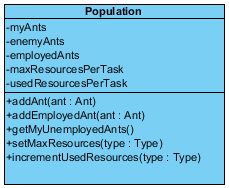
\includegraphics[width=0.5\textwidth]{91_bilder/population}
\caption{Population Klasse}
\label{fig:populationClass}
\end{figure}

Abbildung \ref{fig:populationClass} zeigt unsere Population-Klasse (s. Kapitel \ref{sec:module.Ants.State}), die als zentrale Verwaltungsinstanz f�r unsere Ameisen auch daf�r zust�ndig ist, die allozierten Ressourcen zu verwalten und beim Zuweisen einer Ameise zu einer Aufgabe sicherzustellen, dass das Kontingent nicht �berschritten wird. 

Mit den beiden Feldern \texttt{maxResourcesPerTask} und \texttt{usedResourcesPerTask} wird hier Buch gef�hrt dar�ber, welche Aufgabe wie viele Ameisen verwenden darf, und wie viele sie bereits verwendet hat. Die Aufteilung der Ressourcen, also das Initialisieren von \texttt{maxResourcesPerTask}, geschieht in unserem ResourceAllocator.

\begin{figure}[H]
\centering
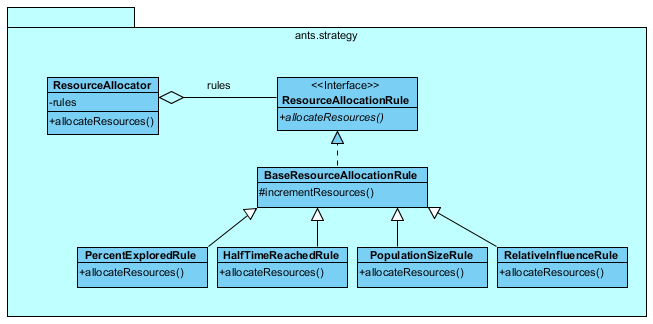
\includegraphics[width=0.9\textwidth]{91_bilder/antsStrategy}
\caption{RessourcenManagement}
\label{fig:antsStrategy}
\end{figure}
 
Abbildung \ref{fig:antsStrategy} zeigt die Klassenhierarchie unserer Ressourcenverwaltung. Die zentrale Klasse ist der ResourceAllocator; mit dessen Methode allocateResources() werden jeweils die Ressourcen neu verteilt:
\lstset{language=Java, tabsize=4}
\begin{lstlisting}
new ResourceAllocator().allocateResources();
\end{lstlisting}
Diese Ressourcenzuteilung wird von unserem Bot jeweils zu Beginn des Zugs vorgenommen. Dazu stellt er als erstes die allozierten Ressourcen pro Aufgabe auf einen definierten Standardwert zur�ck. Diese Werte k�nnen �ber Profile (Kap. \ref{sec:module.Profile}) konfiguriert werden. Dann werden der Reihe nach die konfigurierten Regeln aufgerufen, die jeweils nach ihrer eigenen Logik die Ressourcen f�r bestimmte Aufgaben erh�hen oder verringern. Am Ende entsteht so eine dynamische Ressourcenverteilung, die den verschiedensten Gesichtspunkten Rechnung tragen kann.

\section{Implementierte Regeln}
\label{sec:module.resourceMgmt.Regeln}
Wir haben 4 verschiedene Regeln implementiert, die alle von einer gemeinsamen Basisklasse ableiten. Die Basisklasse \texttt{BaseResourceAllocationRule} stellt die Methode \texttt{incrementResources(Type taskType, int increment, Type... tasksToDecrement)} zur Verf�gung, die ein gegebenes Inkrement (Ressourcen-Plus) f�r eine Aufgabe mit gleichm�ssig verteilten Dekrementen (Ressourcen-Minus) auf die angegebenen anderen Aufgaben ausgleicht.

Unsere implementierten Regeln sind:
\begin{itemize}
	\item \textbf{HalfTimeReachedRule:}	Nach Erreichen der Halbzeit des Spiels sorgt diese Regel daf�r, dass das Angreifen der gegnerischen H�gel h�her priorisiert wird.
	\item \textbf{PercentExploredRule:} Diese Regel sorgt daf�r, dass das Erkunden der Umgebung forciert wird, solange nicht ein gewisser Prozentsatz der Karte bereits erforscht ist.
	\item \textbf{PopulationSizeRule:} Diese Regel forciert die Nahrungsbeschaffung; je nach Gr�sse unseres Ameisenvolks tut sie dies st�rker oder weniger stark.
	\item \textbf{RelativeInfluenceRule:} Fall wir eine dominante Position auf dem Spielfeld haben, sorgt diese Regel f�r zus�tzliche Ressourcen f�r die Erkundung (um das Spielfeld weiter zu kontrollieren) und den Angriff auf gegnerische H�gel.
\end{itemize}
All diese Regeln sind �ber Profile konfigurierbar.

Diese Regeln sind nat�rlich nur eine Auswahl dessen, was mit dieser regelbasierten Ressourcenverwaltung m�glich w�re. Viele weitere Regeln w�ren denkbar, aber wir haben in unseren Tests bereits mit diesen vier einfachen Regeln durchaus zufriedenstellende Ergebnisse erzielt. Eine Schwierigkeit bei der Implementierung neuer Regeln gilt es noch zu beachten: Durch die grosse Dynamik des Systems sind die Auswirkungen einer \"Anderung manchmal nur schwer abzusch�tzen; dieser Effekt wird durch die Konfigurierbarkeit des Systems noch verst�rkt. Die Berechenbarkeit des Verhaltens unseres Bots ist also gr�sser, wenn nicht allzu viele Regeln in die Ressourcenverwaltung eingebunden werden.

